\documentclass[12pt]{article}

% UTF-8 encoding and fonts
\usepackage[utf8]{inputenc}
\usepackage[T1]{fontenc}
\usepackage{lmodern}

% Page setup
\usepackage[margin=1in]{geometry}
\usepackage{setspace}
\onehalfspacing

% Typography
\usepackage{microtype}

% Math and symbols
\usepackage{amsmath,amssymb,amsthm}

% Graphics
\usepackage{graphicx}
\usepackage{float}
\usepackage{subcaption}

% Colors (needed by kableExtra tables)
\usepackage[table]{xcolor}

% Tables
\usepackage{booktabs}
\usepackage{array}
\usepackage{multirow}
\usepackage{threeparttable}
\usepackage{longtable}
\usepackage{pdflscape}
\usepackage{siunitx}
\sisetup{detect-all=true, group-separator={,}, group-minimum-digits=4}
\usepackage{tabularx}

% Bibliography
\usepackage{natbib}
\bibliographystyle{aer}

% Hyperlinks
\usepackage{hyperref}
\hypersetup{
    colorlinks=true,
    linkcolor=blue,
    citecolor=blue,
    urlcolor=blue
}
\usepackage[nameinlink,noabbrev]{cleveref}

% Timing data
\IfFileExists{timing_data.tex}{\input{timing_data.tex}}{
  % Timing macros removed — no execution time data available
}

% Captions
\usepackage{caption}
\captionsetup{font=small,labelfont=bf}

% Section formatting
\usepackage{titlesec}
\titleformat{\section}{\large\bfseries}{\thesection.}{0.5em}{}
\titleformat{\subsection}{\normalsize\bfseries}{\thesubsection}{0.5em}{}

% Euro symbol
\usepackage{textcomp}
\providecommand{\euro}{\texteuro}

% Custom commands
\newcommand{\E}{\mathbb{E}}
\newcommand{\V}{\mathbb{V}}
\newcommand{\rn}{Rassemblement National}
\newcommand{\fn}{Front National}
\newcommand{\gj}{\textit{Gilets Jaunes}}
\newcommand{\dept}{d\'{e}partement}
\newcommand{\depts}{d\'{e}partements}

\begin{document}

%% ===================================================================
%%  TITLE PAGE
%% ===================================================================

\begin{titlepage}
\begin{center}
\vspace*{1cm}

{\LARGE\bfseries Connected Backlash: Social Networks and the\\
Political Economy of Carbon Taxation in France}

\vspace{1cm}

{\large APEP Working Paper apep\_0464\_v2\footnote{This paper is a revision of APEP-0464. See \url{https://github.com/SocialCatalystLab/ape-papers/tree/main/apep_0464} for the original. All analysis conducted in R; replication code and data are available in the paper repository.}}

\vspace{0.5cm}

{\large February 2026}

\vspace{1cm}

\begin{abstract}
\noindent On November 17, 2018, 300,000 French citizens donned yellow vests to protest a carbon tax---but the protests spread far beyond where the tax hit hardest. This paper shows that social networks transmitted the backlash. Using Facebook's Social Connectedness Index to measure ties between French \depts{}, I construct commune-level network exposure to fuel-vulnerable communities. In a panel of 37,000 communes across ten elections (2002--2024), network exposure raises \rn{} vote share by 1.19 percentage points per standard deviation---67\% larger than a commune's own fuel costs. An event study with four pre-treatment coefficients confirms flat pre-trends. The effect is absent for Green and center-right parties, strongest in rural areas, and robust to distance restrictions isolating social from geographic proximity. A spatial autoregressive model estimates that a one-percentage-point localized shock propagates to a nationally-weighted 2.4-percentage-point effect through network amplification.
\end{abstract}

\vspace{0.3cm}

\textbf{JEL Codes:} D72, H23, Q54, L14, R41

\textbf{Keywords:} Carbon tax, social networks, populism, political economy, France, \textit{Gilets Jaunes}

\end{center}
\end{titlepage}


%% ===================================================================
%%  INTRODUCTION
%% ===================================================================

\section{Introduction}
\label{sec:intro}

On a Saturday morning in November 2018, traffic circles across France filled with people wearing high-visibility vests. The \gj{} movement---named after the safety vests French drivers must carry---erupted in response to a carbon tax increase that would have raised diesel prices by about four centimes per liter. Within weeks, the protests had spread to every \dept{} in metropolitan France, drawn hundreds of thousands of participants, and forced President Macron to freeze the tax at \euro 44.60 per ton of CO\textsubscript{2}.

The puzzle is not that people protested a tax increase. The puzzle is \emph{where} they protested. The \gj{} movement was most intense not in the handful of \depts{} where long commutes and diesel dependence made the tax most painful, but in a broad swath of semi-rural France where the direct cost was modest. Something was transmitting the grievance beyond its economic footprint.

This paper shows that social networks are the transmission mechanism. I measure the structure of social ties between French \depts{} using Facebook's Social Connectedness Index (SCI), a dataset that captures the probability that two randomly chosen users in different regions are friends on Facebook. I combine these network weights with \dept{}-level fuel vulnerability---measured by commuting CO\textsubscript{2} emissions per worker---to construct a commune-level index of \emph{network exposure} to the carbon tax. The question is whether a commune's political response depends not only on its own fuel costs, but also on the fuel costs borne by the people its residents are connected to.

The answer is yes, and the network channel dominates. In a panel of approximately 37,000 communes observed across ten national elections from 2002 to 2024, I estimate that a one-standard-deviation increase in network fuel exposure raises the \rn{} first-round vote share by 1.19 percentage points in the post-carbon-tax period. The effect of a commune's own fuel vulnerability is smaller: 0.72 percentage points. Network exposure---what your friends experience---matters 67\% more than direct exposure for predicting populist voting.

The identification strategy is a shift-share design in the tradition of \citet{goldsmith2020bartik} and \citet{borusyak2022quasi}. The ``shares'' are pre-existing SCI network weights that capture historical social connections. The ``shifts'' are \dept{}-level fuel vulnerability scores derived from commuting patterns and vehicle fleet composition---variation that is plausibly exogenous to political preferences conditional on own fuel costs. The key identifying assumption is that, conditional on a commune's own fuel vulnerability and commune and election fixed effects, the SCI-weighted average of other \depts{}' fuel vulnerability is uncorrelated with unobserved determinants of \rn{} support.

Four features of the research design support this assumption. First, an event study spanning ten elections---five before and five after the carbon tax introduction in 2014---shows that network exposure had no differential relationship with \rn{} support during the pre-treatment period. The pre-treatment coefficients are tightly clustered near zero, with the break occurring precisely at the 2014 European election when the carbon tax was enacted at \euro 7 per ton of CO\textsubscript{2}. Second, I exploit the continuous variation in the carbon tax rate itself, which rose from zero to \euro 44.60 across the sample period, providing four distinct dose levels rather than a binary pre/post comparison. Each \euro 10 increase in the carbon rate amplifies the network effect by 0.31 percentage points. Third, restricting the SCI matrix to department pairs separated by more than 200 kilometers---eliminating geographic neighbors who might share local labor markets---preserves the network effect. Fourth, placebo outcomes confirm that the mechanism is specific to anti-tax populism: network fuel exposure has no effect on support for Green or center-right parties.

A structural spatial autoregressive model allows me to quantify the total network multiplier. The estimated spatial parameter $\hat{\rho} = 0.955$ implies that a localized one-percentage-point shock to \rn{} support in a single \dept{} is amplified roughly 2.4-fold through the equilibrium network process. To assess whether $\rho$ captures genuine network contagion or merely spatially correlated errors, I estimate a spatial error model (SEM) and a spatial Durbin model (SDM) following the approach of \citet{lesage2009introduction}. The SEM produces a similarly high spatial parameter ($\hat{\lambda} = 0.939$), meaning I cannot rule out correlated shocks as an alternative explanation. But a likelihood ratio test comparing the SAR and SDM finds no evidence that spillover covariates ($WX$) improve the fit ($p = 0.506$), supporting the more parsimonious SAR specification.

This paper contributes to three literatures. The first studies the political economy of climate policy \citep{douenne2022yellow, klenert2018carbon, stantcheva2022understanding}. The existing evidence focuses on how direct economic costs shape policy preferences. I show that network exposure may matter more than direct costs, which implies that the political feasibility of carbon pricing depends not just on how many people are hurt, but on how connected those people are to the rest of the polity.

The second literature examines the economic roots of populism \citep{autor2013china, colantone2018trade, fetzer2019did, rodrik2021populism, funke2016going, guiso2019global}. These papers typically identify local economic shocks---trade exposure, austerity, financial crises---and trace their effects on voting. My contribution is to show that the political response to an economic shock propagates through social networks, reaching communities that were not directly affected. The implication is that standard models of economic voting, which condition on local conditions alone, underestimate the political fallout from geographically concentrated shocks.

The third literature studies social networks and political behavior \citep{fluckiger2025bro, enikolopov2020social, halberstam2016homophily, bailey2018social, chetty2022social1}. I contribute a clean empirical setting where the timing and geography of the economic shock are known, network structure is observed (not inferred from behavior), and the political outcome is measured in high-stakes elections with near-universal participation. The carbon tax provides a rare case where the policy's incidence varies geographically in a measurable way, allowing me to identify the network channel without relying on arbitrary proximity measures.

Several methodological features distinguish this paper. The expanded panel with five pre-treatment elections (2002--2012), yielding four estimable pre-treatment coefficients relative to the 2012 baseline, provides a stronger test of parallel trends than is typical in the political economy literature, where most DiD designs rely on one or two pre-periods. The continuous treatment specification, which exploits the sixfold variation in the carbon rate from \euro 7 to \euro 44.60, provides a dose-response test that is not susceptible to confounding by ``post-2017 politics'' more broadly. The spatial model comparison (SAR vs.\ SEM vs.\ SDM) follows best practices in spatial econometrics \citep{lesage2009introduction, anselin1988spatial} and provides an honest assessment of the structural interpretation's limits. And the placebo party outcomes (Green and center-right) test the mechanism's specificity in a way that goes beyond standard robustness.

Section~\ref{sec:background} describes the institutional background. Sections~\ref{sec:framework}--\ref{sec:strategy} lay out the framework, data, and empirical strategy. Sections~\ref{sec:results}--\ref{sec:robustness} present results. Section~\ref{sec:discussion} interprets the findings.


%% ===================================================================
%%  INSTITUTIONAL BACKGROUND
%% ===================================================================

\section{Institutional Background}
\label{sec:background}

\subsection{The French Carbon Tax}

France introduced a carbon tax (\textit{Contribution Climat-\'{E}nergie}, CCE) as part of the 2014 Finance Act, enacted in December 2013 and taking effect on January 1, 2014. The tax was embedded in the existing energy excise (\textit{Taxe Int\'{e}rieure de Consommation sur les Produits \'{E}nerg\'{e}tiques}, TICPE) by linking a portion of the rate to the CO\textsubscript{2} content of fossil fuels. The initial rate was \euro 7 per ton of CO\textsubscript{2} in 2014, rising through a pre-announced schedule: \euro 14.50 in 2015, \euro 22 in 2016, \euro 30.50 in 2017, and \euro 44.60 in 2018. The first ``treated'' election in my sample is the May 2014 European election, by which point voters had been paying the carbon tax for approximately five months.

The tax fell disproportionately on diesel, which accounted for roughly 80\% of road fuel consumption in France. For a household commuting by car, the tax at its 2018 rate added approximately \euro 120 per year in fuel costs---a modest sum in absolute terms but a visible one, printed on every gas station receipt. \citet{bureau2019distributional} show that the incidence was regressive in spatial terms: rural households with long commutes and limited public transit alternatives bore a share of the burden far exceeding their share of emissions.

The scheduled increase to \euro 55 per ton in 2019 was the proximate trigger of the \gj{} protests. The government froze the rate at \euro 44.60 in December 2018. It has remained at that level through 2024.

\subsection{The \textit{Gilets Jaunes}}

The \gj{} movement began with an online petition in May 2018 opposing fuel price increases. The first national day of action on November 17, 2018, drew approximately 300,000 participants who blocked traffic circles (\textit{ronds-points}) across France. The movement was notable for its geographic diffusion: while Paris drew the most media coverage, the largest participation rates were in small towns and rural areas where car dependence was highest.

The movement had no formal organization or leadership, which makes it a useful natural experiment: political mobilization was driven by economic grievance and social diffusion rather than top-down party strategy. The \rn{} was the primary electoral beneficiary. Marine Le Pen's party had already been gaining vote share throughout the 2010s, but the \gj{} protests accelerated the trend in fuel-vulnerable areas.

\subsection{The \rn{} and French Elections}

The \rn{} (formerly \fn{}) has contested every presidential and European election since its founding in 1972. Under Jean-Marie Le Pen, the party won 17.3\% in the 2002 presidential first round (averaged across communes in my data), shocking France by advancing to the runoff. Support declined under internal turmoil to 12.5\% in 2007 and 7.6\% in the 2009 European election. Marine Le Pen's rebranding beginning in 2011 revived the party: it won 21.2\% in 2012, surged to 29.2\% in the 2014 European election, and reached 38.3\% in the 2024 European election.

The party's geographic base shifted over this period. In the 2002 presidential election, \fn{} support was concentrated in the Mediterranean coast and industrial northeast---the party's traditional bastions. By 2024, the \rn{} had become the dominant party in rural and periurban France, gaining most in the \depts{} where car dependence is highest and public transit coverage is lowest. This geographic reorientation coincides precisely with the carbon tax era, providing the motivating variation for this paper.

The ten elections in my panel (five presidential first rounds: 2002, 2007, 2012, 2017, 2022; five European: 2004, 2009, 2014, 2019, 2024) span this entire trajectory. The five elections before 2014 provide a clean pre-treatment period when the carbon tax did not exist. Importantly, the pre-treatment period includes both periods of \fn{} strength (2002) and weakness (2009), allowing me to test whether the network channel operates specifically in the carbon-tax era or was already present during earlier \fn{} fluctuations.


%% ===================================================================
%%  CONCEPTUAL FRAMEWORK
%% ===================================================================

\section{Conceptual Framework}
\label{sec:framework}

I model political opinion formation as a DeGroot learning process on the social network \citep{degroot1974reaching, golub2010naive}. Each agent $i$ holds a political attitude $y_i$ (propensity to vote \rn{}) that depends on the agent's own economic circumstances and on the attitudes of friends. In each period, agents update their views by taking a weighted average of their neighbors' attitudes:
\begin{equation}
y_i^{(t+1)} = (1 - \alpha) y_i^{(0)} + \alpha \sum_j w_{ij} y_j^{(t)},
\label{eq:degroot}
\end{equation}
where $y_i^{(0)}$ is the agent's ``fundamental'' political leaning, $w_{ij}$ is the network weight (SCI-based), and $\alpha \in (0,1)$ governs the strength of social influence. The fundamental $y_i^{(0)}$ depends on the carbon tax burden: communes with high fuel vulnerability and those connected to fuel-vulnerable friends form more negative attitudes toward the governing coalition.

At the steady state, the vector of attitudes is:
\begin{equation}
\mathbf{y}^* = (I - \alpha W)^{-1} (1-\alpha) \mathbf{y}^{(0)}.
\label{eq:steady_state}
\end{equation}

This is the reduced-form of the spatial autoregressive model $\mathbf{y} = \rho W \mathbf{y} + X\beta + \varepsilon$ with $\rho = \alpha$. The matrix $(I - \rho W)^{-1}$ is the ``network multiplier'': a local shock to one node reverberates through the network, affecting all connected nodes with intensity proportional to network distance.

Two testable predictions follow. First, communes with greater network exposure to fuel-vulnerable \depts{} should show higher \rn{} support after the carbon tax, \emph{controlling for own fuel vulnerability}. Second, the total effect of fuel vulnerability on political outcomes should exceed the direct effect---the network multiplier should be greater than one.

The framework also clarifies what the SEM alternative captures. If $\rho$ reflects genuine social influence (friends' grievances change your vote), the SAR model is correct. If instead the spatial correlation arises because connected regions share unobserved shocks (e.g., media exposure, local political events), the SEM $\mathbf{y} = X\beta + u$, $u = \lambda W u + \varepsilon$ is more appropriate. I estimate both models in Section~\ref{sec:structural}.


%% ===================================================================
%%  DATA
%% ===================================================================

\section{Data}
\label{sec:data}

\subsection{Elections}

I use first-round results from ten national elections held between 2002 and 2024, obtained from data.gouv.fr. Five are presidential elections (2002, 2007, 2012, 2017, 2022) and five are European Parliament elections (2004, 2009, 2014, 2019, 2024). For each of approximately 37,000 communes, I compute the \rn{}/\fn{} vote share as a percentage of valid ballots cast. Party identification accounts for the renaming from \fn{} to \rn{} in 2018 and for list-based voting in European elections. I also compute vote shares for Green parties (EELV/VEC and allied lists) and center-right parties (UMP/LR) as placebo outcomes.

\subsection{Social Connectedness Index}

The SCI, developed by \citet{bailey2018social} and made available by Facebook (now Meta), measures the relative probability that users in two regions are friends. I use the NUTS-3 version, which maps to French \depts{} for metropolitan France (96 units). For each pair of \depts{} $(d, d')$, the SCI is:
\begin{equation}
\text{SCI}_{dd'} = \frac{\text{FB friends}_{dd'}}{\text{FB users}_d \times \text{FB users}_{d'}},
\end{equation}
capturing the density of social connections. I row-normalize the SCI matrix so that each \dept{}'s outgoing weights sum to one.

\subsection{Fuel Vulnerability}

I construct \dept{}-level fuel vulnerability from the INSEE \textit{Base Carbone} commuting database, which records CO\textsubscript{2} emissions from home-to-work travel. The variable $\text{CO2}_{d}$ is the average annual CO\textsubscript{2} per commuter (in tons) in \dept{} $d$. Departments with long commutes, low public transit coverage, and diesel-heavy vehicle fleets score highest. The most fuel-vulnerable \dept{} (Ain, 0.93 tCO\textsubscript{2}/commuter) is roughly three times more exposed than the least vulnerable (Paris, 0.30).

The geographic pattern of fuel vulnerability reflects France's urban structure. The \^{I}le-de-France region (Paris and suburbs) has the lowest commuting emissions thanks to the Metro, RER, and dense bus networks. The rural \depts{} of central France---Creuse, Cantal, Loz\`{e}re---have the highest per-commuter emissions because workers travel long distances on roads with no public transit alternatives. The industrial north and northeast occupy an intermediate position: commuting distances are shorter but car dependence is high. Figure~\ref{fig:map_fuel} maps this variation.

\begin{figure}[H]
\centering
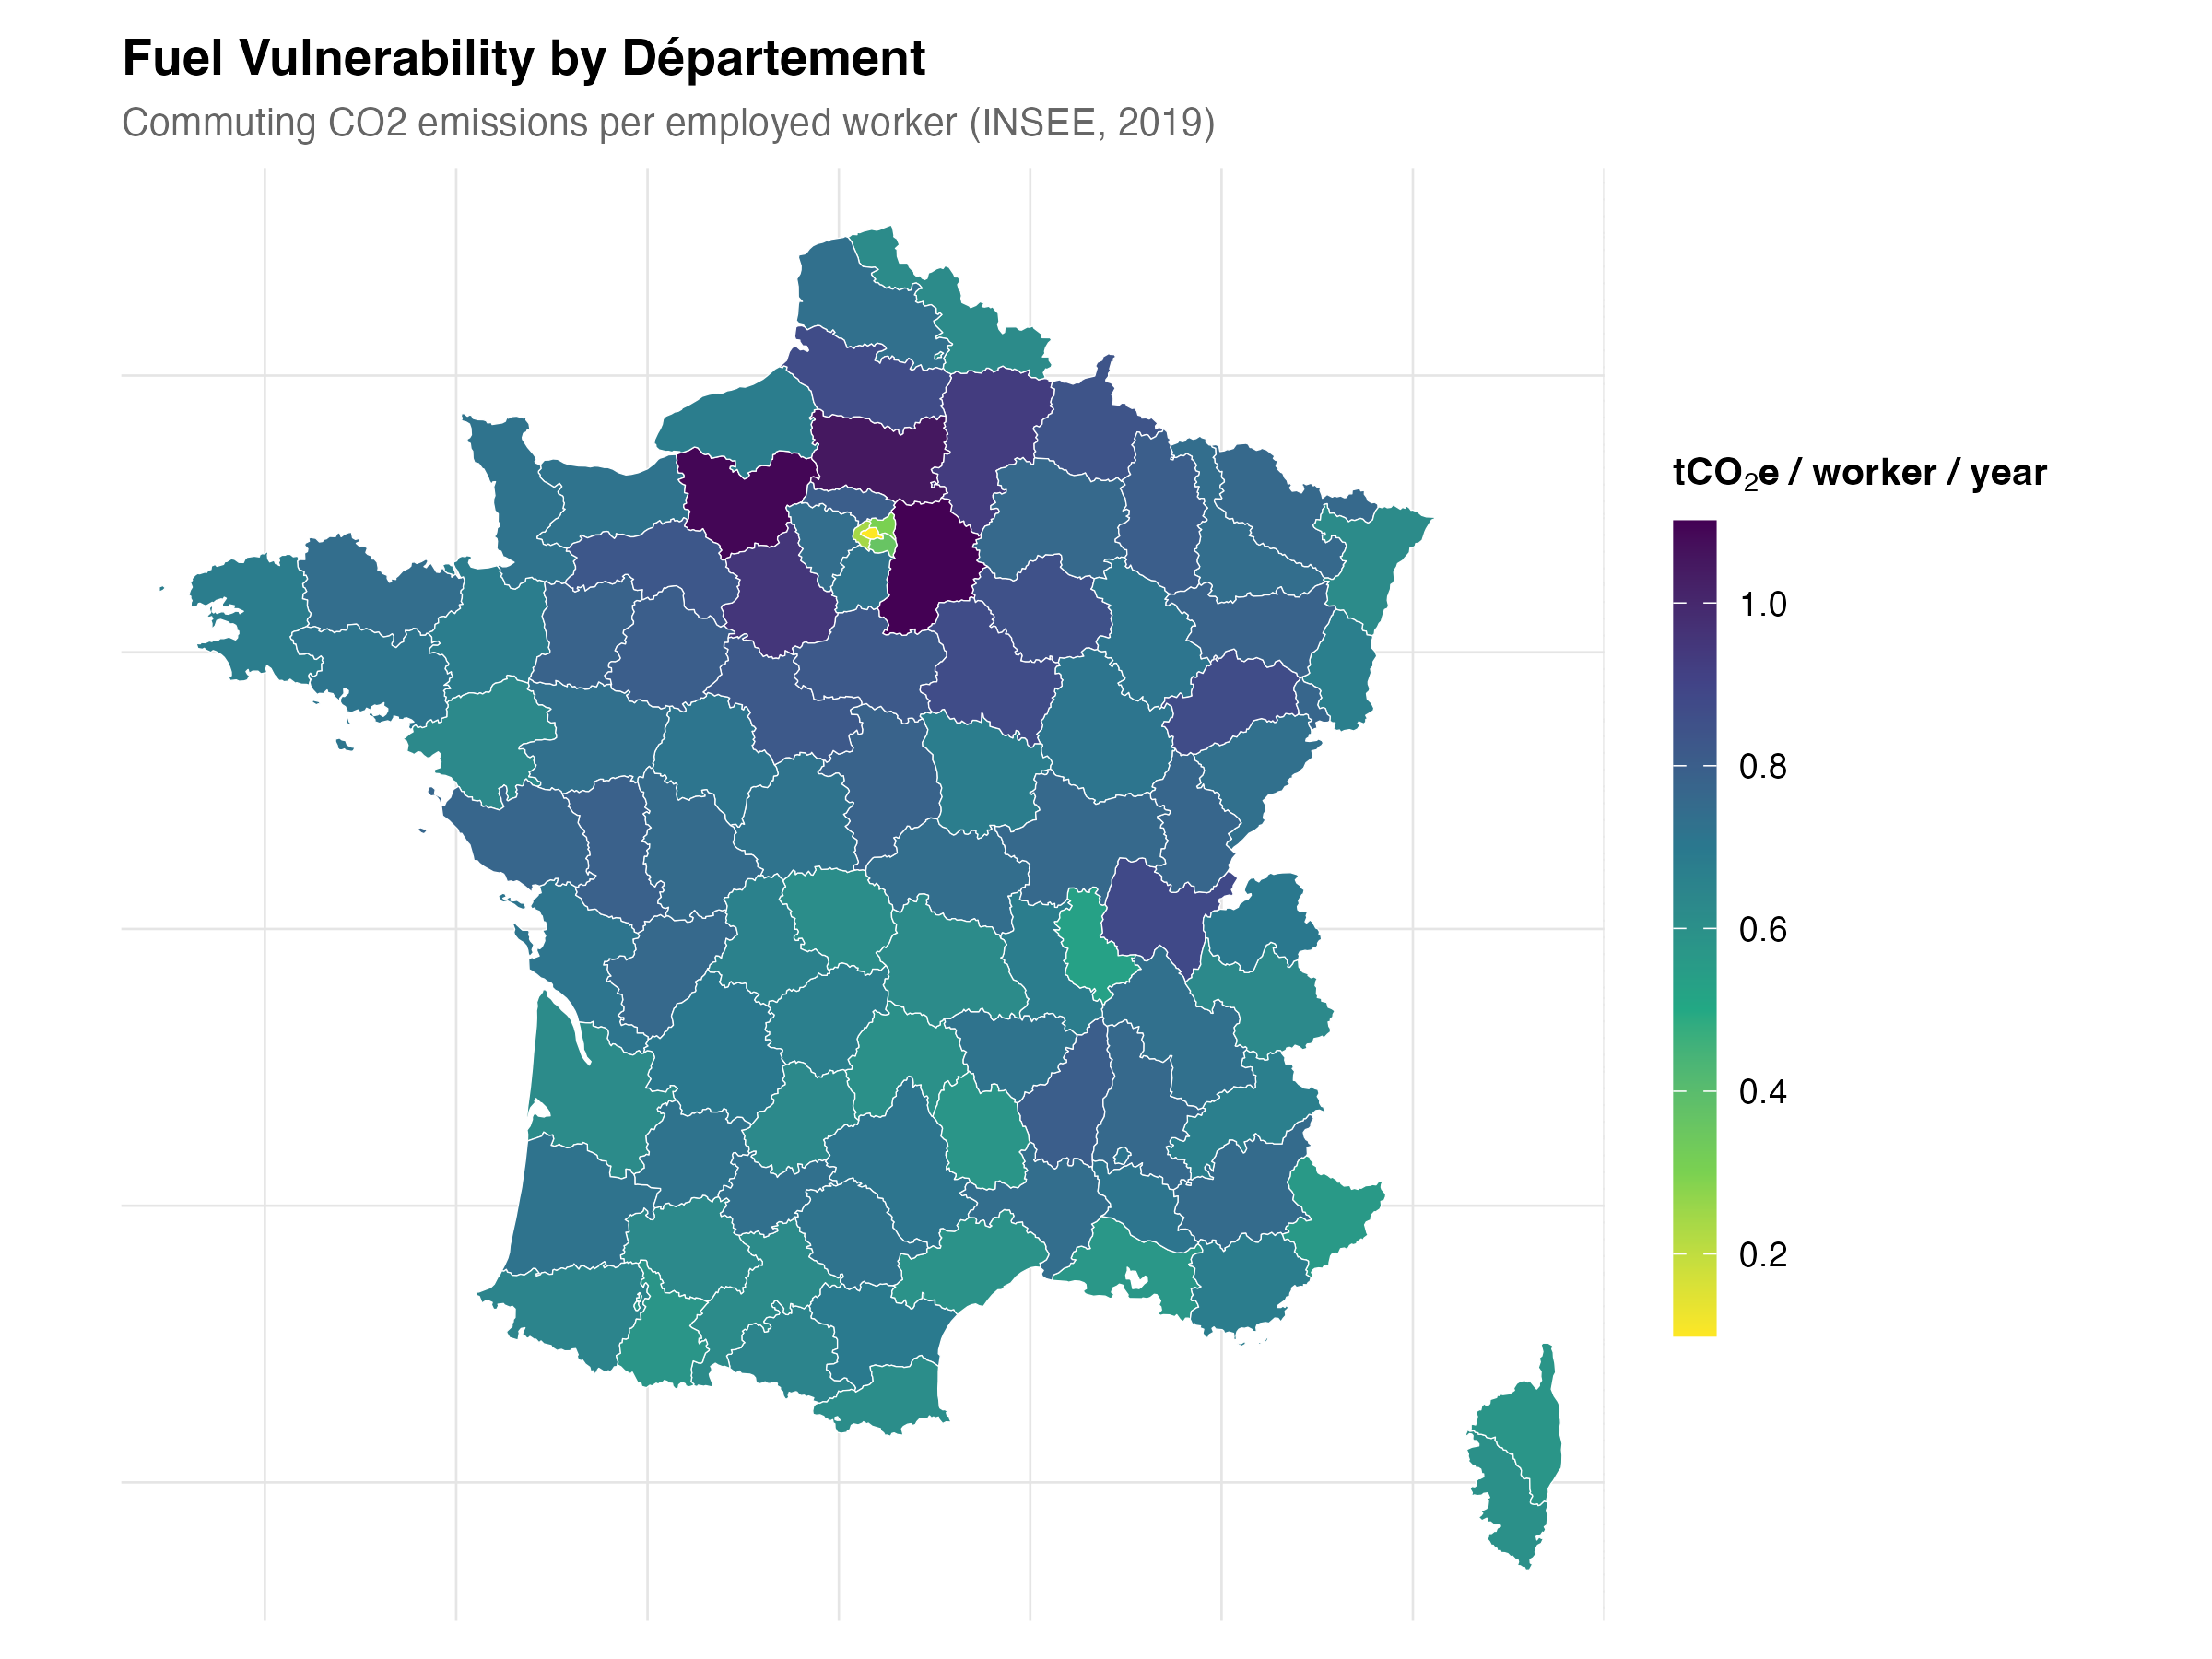
\includegraphics[width=0.8\textwidth]{figures/fig_map_fuel_vulnerability.png}
\caption{Fuel Vulnerability by D\'{e}partement}
\label{fig:map_fuel}
\begin{minipage}{\textwidth}
\small
\textit{Notes:} Average commuting CO\textsubscript{2} emissions per employed worker (tCO\textsubscript{2}/year) from INSEE Base Carbone. Darker colors indicate higher fuel vulnerability. Metropolitan France only (96 \depts{}).
\end{minipage}
\end{figure}

The SCI-weighted network exposure (Equation~\ref{eq:network_exposure}) captures a different geographic pattern. While own fuel vulnerability is highest in rural central France, network fuel exposure is more evenly distributed because social connections span geographic distance. A \dept{} like Seine-Saint-Denis (low own exposure, suburban Paris) can have high network exposure because its residents are connected to fuel-vulnerable relatives in Picardy and Normandy. Figure~\ref{fig:map_net} shows that network exposure varies less than own exposure but follows a distinct geographic pattern, with the highest values in the northern industrial belt.

\begin{figure}[H]
\centering
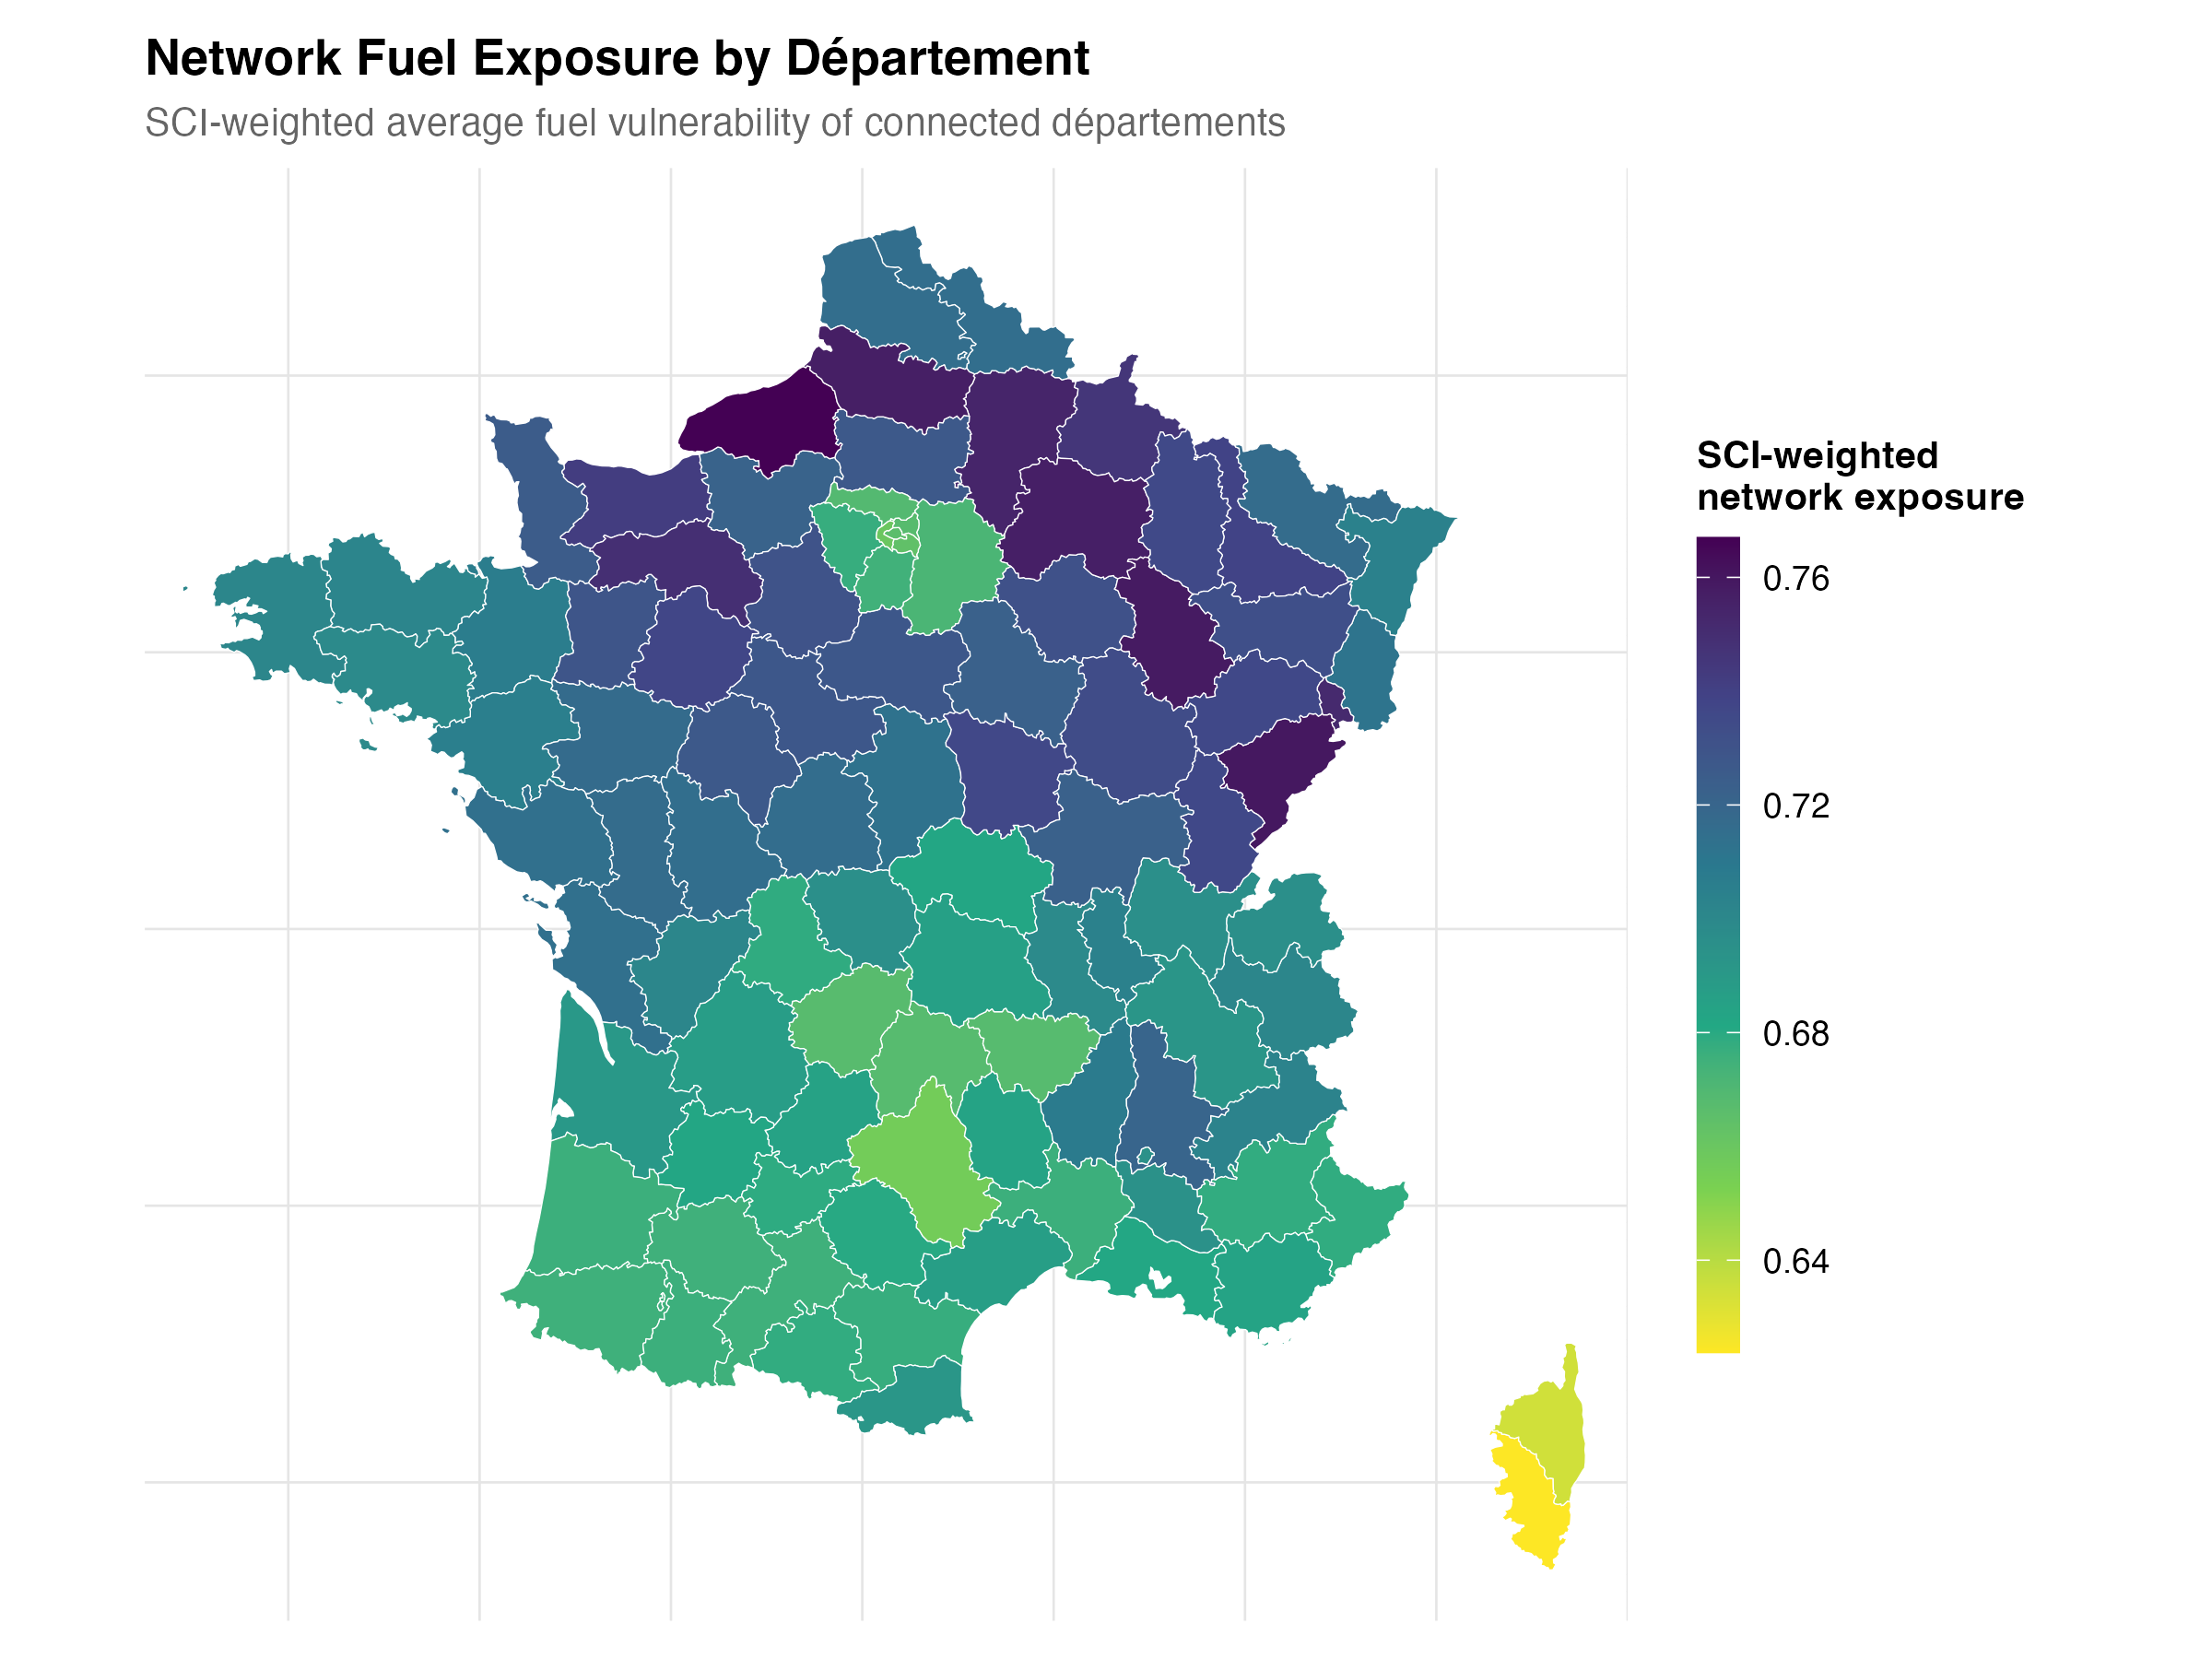
\includegraphics[width=0.8\textwidth]{figures/fig_map_network_exposure.png}
\caption{Network Fuel Exposure by D\'{e}partement}
\label{fig:map_net}
\begin{minipage}{\textwidth}
\small
\textit{Notes:} SCI-weighted average of other \depts{}' fuel vulnerability, excluding own \dept{}. Row-normalized SCI weights. Higher values indicate stronger social connections to fuel-vulnerable areas.
\end{minipage}
\end{figure}

\subsection{Variable Construction}

For each commune $c$ in \dept{} $d$, I construct two exposure measures:

\textbf{Own fuel exposure.} The standardized CO\textsubscript{2} commuting intensity of the commune's own \dept{}: $\text{Own}_d = (\text{CO2}_d - \bar{\text{CO2}}) / \sigma_{\text{CO2}}$.

\textbf{Network fuel exposure.} The SCI-weighted average of other \depts{}' fuel vulnerability, excluding $d$ itself:
\begin{equation}
\text{Net}_d = \frac{\sum_{d' \neq d} \text{SCI}_{dd'} \times \text{CO2}_{d'}}{\sum_{d' \neq d} \text{SCI}_{dd'}},
\label{eq:network_exposure}
\end{equation}
also standardized. This is the shift-share instrument: SCI weights (shares) interact with fuel vulnerability (shifts).

\textbf{Carbon tax rate.} The tax rate $R_t$ varies across the sample: $R_t = 0$ for 2002--2012, $R_t = 7$ for 2014, $R_t = 30.5$ for 2017, $R_t = 44.6$ for 2019--2024 (in \euro/tCO\textsubscript{2}).

\subsection{Summary Statistics}

The final commune-level panel contains 361,796 commune-election observations (approximately 37,000 communes $\times$ 10 elections, with minor attrition from commune mergers and missing data). Table~\ref{tab:summary} reports summary statistics.

\begin{table}[H]
\centering
\caption{Summary Statistics}
\label{tab:summary}
\begin{threeparttable}
\begin{tabular}{@{}lrrrr@{}}
\toprule
Variable & Mean & SD & Min & Max \\
\midrule
\rn{} vote share (\%) & 22.07 & 11.76 & 0.00 & 100.00 \\
Turnout (\%) & 65.12 & 14.83 & 0.00 & 100.00 \\
Own CO\textsubscript{2} (tCO\textsubscript{2}/commuter, raw) & 0.72 & 0.13 & 0.30 & 1.10 \\
Network fuel exposure (raw) & 0.73 & 0.02 & 0.64 & 0.82 \\
Carbon rate (\euro/tCO\textsubscript{2}) & 17.10 & 20.29 & 0.00 & 44.60 \\
\bottomrule
\end{tabular}
\begin{tablenotes}
\small
\item \textit{Notes:} Commune-election level. $N = 361{,}796$ observations across 10 elections (2002--2024). \rn{} vote share is the first-round \fn{}/\rn{} share of valid ballots. Own CO\textsubscript{2} and Network fuel exposure are reported in raw (unstandardized) units; in regressions, both are standardized to mean zero, unit variance within the estimation sample.
\end{tablenotes}
\end{threeparttable}
\end{table}


%% ===================================================================
%%  EMPIRICAL STRATEGY
%% ===================================================================

\section{Empirical Strategy}
\label{sec:strategy}

\subsection{Main Specification}

I estimate the effect of own and network fuel exposure on \rn{} vote share using a two-way fixed effects model:
\begin{equation}
\text{RN}_{ct} = \alpha_c + \gamma_t + \beta_1 (\text{Own}_d \times \text{Post}_t) + \beta_2 (\text{Net}_d \times \text{Post}_t) + \varepsilon_{ct},
\label{eq:main}
\end{equation}
where $c$ indexes communes, $t$ indexes elections, $d$ denotes the \dept{} containing commune $c$, $\alpha_c$ is a commune fixed effect, $\gamma_t$ is an election fixed effect, and $\text{Post}_t$ equals one for elections from 2014 onward (when the carbon tax was in effect). Standard errors are clustered at the \dept{} level (96 clusters).

The commune fixed effect absorbs all time-invariant commune characteristics (geography, demographics, historical voting patterns). The election fixed effect absorbs national trends (the \rn{}'s secular rise, national economic conditions, candidate quality). The coefficient $\beta_2$ identifies the network effect from \emph{within-commune, within-election} variation: among communes that share the same national environment and the same permanent characteristics, do those with greater network exposure to fuel-vulnerable \depts{} show larger \rn{} gains after the carbon tax?

\textbf{Effective sample size.} Although the commune-election panel contains 361,796 observations, both $\text{Own}_d$ and $\text{Net}_d$ vary only at the \dept{} level. The identifying variation is therefore at the level of 96 \depts{} $\times$ 10 elections = 960 cells, and the commune panel provides repeated observations of the same treatment within each cell. Standard errors are clustered at the \dept{} level to account for this. I also present \dept{}-level regressions (Table~\ref{tab:dept}, $N = 960$) as a complementary analysis that operates at the same level as the identifying variation, and an inference comparison (Table~\ref{tab:inference}) that includes wild cluster bootstrap and randomization inference to probe sensitivity to the clustering structure.

\subsection{Continuous Treatment}

The binary $\text{Post}_t$ indicator pools elections at four different tax rates (\euro 0, 7, 30.5, 44.6). I also estimate a continuous specification:
\begin{equation}
\text{RN}_{ct} = \alpha_c + \gamma_t + \beta_1 (\text{Own}_d \times R_t) + \beta_2 (\text{Net}_d \times R_t) + \varepsilon_{ct},
\label{eq:continuous}
\end{equation}
where $R_t$ is the carbon tax rate in \euro/tCO\textsubscript{2}. This specification exploits the variation in the tax rate across elections: $R_t = 0$ for five pre-treatment elections, $R_t = 7$ in 2014, $R_t = 30.5$ in 2017, and $R_t = 44.6$ for 2019--2024. The dose-response test is: if the network effect is driven by the carbon tax, it should increase with the rate.

\subsection{Event Study}

To test the parallel trends assumption, I estimate an event study interacting fuel exposure with indicators for each election, using the 2012 presidential election (the last pre-carbon-tax election) as the reference:
\begin{equation}
\text{RN}_{ct} = \alpha_c + \gamma_t + \sum_{k \neq 2012} \delta^{\text{own}}_k (\text{Own}_d \times \mathbf{1}[t = k]) + \sum_{k \neq 2012} \delta^{\text{net}}_k (\text{Net}_d \times \mathbf{1}[t = k]) + \varepsilon_{ct}.
\label{eq:event_study}
\end{equation}
Figure~\ref{fig:event_study} plots both sets of coefficients. Parallel trends requires $\delta^{\text{net}}_k \approx 0$ for $k \in \{2002, 2004, 2007, 2009\}$: before the carbon tax, network fuel exposure should not predict differential changes in \rn{} support. The post-treatment coefficients $\delta^{\text{net}}_k$ for $k \in \{2014, 2017, 2019, 2022, 2024\}$ trace out the dynamic treatment effect.

\subsection{Threats to Identification}

The main threat is that SCI-weighted fuel vulnerability correlates with unobserved determinants of \rn{} support that change differentially over time. Three arguments mitigate this concern.

First, the event study provides a direct test: if the parallel trends assumption fails, the pre-treatment coefficients will be non-zero. Second, the SCI captures \emph{social} proximity, not geographic proximity. By restricting the network to \dept{} pairs more than 200 km apart, I can isolate social connections from shared local shocks \citep{bailey2020social}. Third, the shift-share structure means that $\beta_2$ is identified even if SCI weights are endogenous, provided the \dept{}-level fuel vulnerability ``shifts'' are exogenous---a condition that holds if commuting patterns are determined by geography and infrastructure rather than political preferences \citep{borusyak2022quasi}.


%% ===================================================================
%%  RESULTS
%% ===================================================================

\section{Results}
\label{sec:results}

\subsection{Main Estimates}

Table~\ref{tab:main} presents the main results. In Model 1, own fuel exposure alone raises \rn{} vote share by 0.72 percentage points per standard deviation after the carbon tax ($p < 0.001$). But in Model 2, network exposure enters with a coefficient of 1.19 percentage points---67\% larger. When both enter simultaneously (Model 3), both remain significant: the own-exposure effect is 0.72 pp (SE = 0.18) and the network effect is 1.19 pp (SE = 0.24). The network effect is not crowding out the own effect; both channels operate independently.

\begin{table}[H]
\centering
\caption{Main Results: \rn{} Vote Share and Carbon Tax Exposure}
\label{tab:main}
\begin{threeparttable}
\begin{tabular}{@{}lcccccc@{}}
\toprule
 & (1) & (2) & (3) & (4) & (5) & (6) \\
 & Own & Network & Both & Post-GJ & Pres$\times$Euro & Continuous \\
\midrule
Own $\times$ Post & 0.716$^{***}$ & & 0.716$^{***}$ & 0.698$^{***}$ & 0.888$^{***}$ & \\
 & (0.183) & & (0.183) & (0.196) & (0.221) & \\[3pt]
Net $\times$ Post & & 1.192$^{***}$ & 1.192$^{***}$ & 1.067$^{***}$ & 1.137$^{***}$ & \\
 & & (0.237) & (0.237) & (0.244) & (0.280) & \\[3pt]
Own $\times$ Post $\times$ Pres & & & & & $-$0.344$^{***}$ & \\
 & & & & & (0.102) & \\[3pt]
Net $\times$ Post $\times$ Pres & & & & & 0.111 & \\
 & & & & & (0.116) & \\[3pt]
Own $\times$ Rate & & & & & & 0.020$^{***}$ \\
 & & & & & & (0.005) \\[3pt]
Net $\times$ Rate & & & & & & 0.031$^{***}$ \\
 & & & & & & (0.006) \\[3pt]
\midrule
Commune FE & Yes & Yes & Yes & Yes & Yes & Yes \\
Election FE & Yes & Yes & Yes & Yes & Yes & Yes \\
$N$ & 361,796 & 361,796 & 361,796 & 361,796 & 361,796 & 361,796 \\
\bottomrule
\end{tabular}
\begin{tablenotes}
\small
\item \textit{Notes:} Dependent variable is \rn{}/\fn{} first-round vote share (\%). Own and Net are standardized \dept{}-level fuel vulnerability (own and SCI-weighted network average). Post = 1 for elections from 2014 onward. Rate is the carbon tax rate in \euro/tCO\textsubscript{2}. Standard errors clustered by \dept{} in parentheses. $^{***}p<0.01$, $^{**}p<0.05$, $^{*}p<0.10$.
\end{tablenotes}
\end{threeparttable}
\end{table}

Model 4 restricts the treatment period to post-\gj{} elections (2019 onward). The network coefficient falls slightly to 1.07 pp, suggesting that most of the effect was already present at the carbon tax's introduction, before the protests amplified it. Model 5 interacts treatment with election type. The network effect is statistically indistinguishable across presidential and European elections ($p = 0.34$ for the interaction), confirming that the result is not driven by a single election format.

The continuous specification (Model 6) is the most demanding test. Each \euro 10 increase in the carbon rate amplifies the network effect by 0.31 pp (SE = 0.06) and the own effect by 0.20 pp (SE = 0.05). At the 2018 rate of \euro 44.60, the implied network effect is $0.031 \times 44.6 = 1.38$ pp per standard deviation of network exposure---closely matching the binary estimate of 1.19 pp.

\subsection{Event Study}

Figure~\ref{fig:event_study} plots the event study coefficients for network exposure, with the 2012 presidential election as the reference period. The pattern is striking. During the pre-treatment period, with 2012 as the reference, the four estimated pre-treatment coefficients (2002, 2004, 2007, 2009) are clustered near zero: the largest is $-0.48$ (2002, SE = 0.24), and three of four are statistically insignificant. Network fuel exposure had no systematic relationship with differential \rn{} trends before the carbon tax existed.

\begin{figure}[H]
\centering
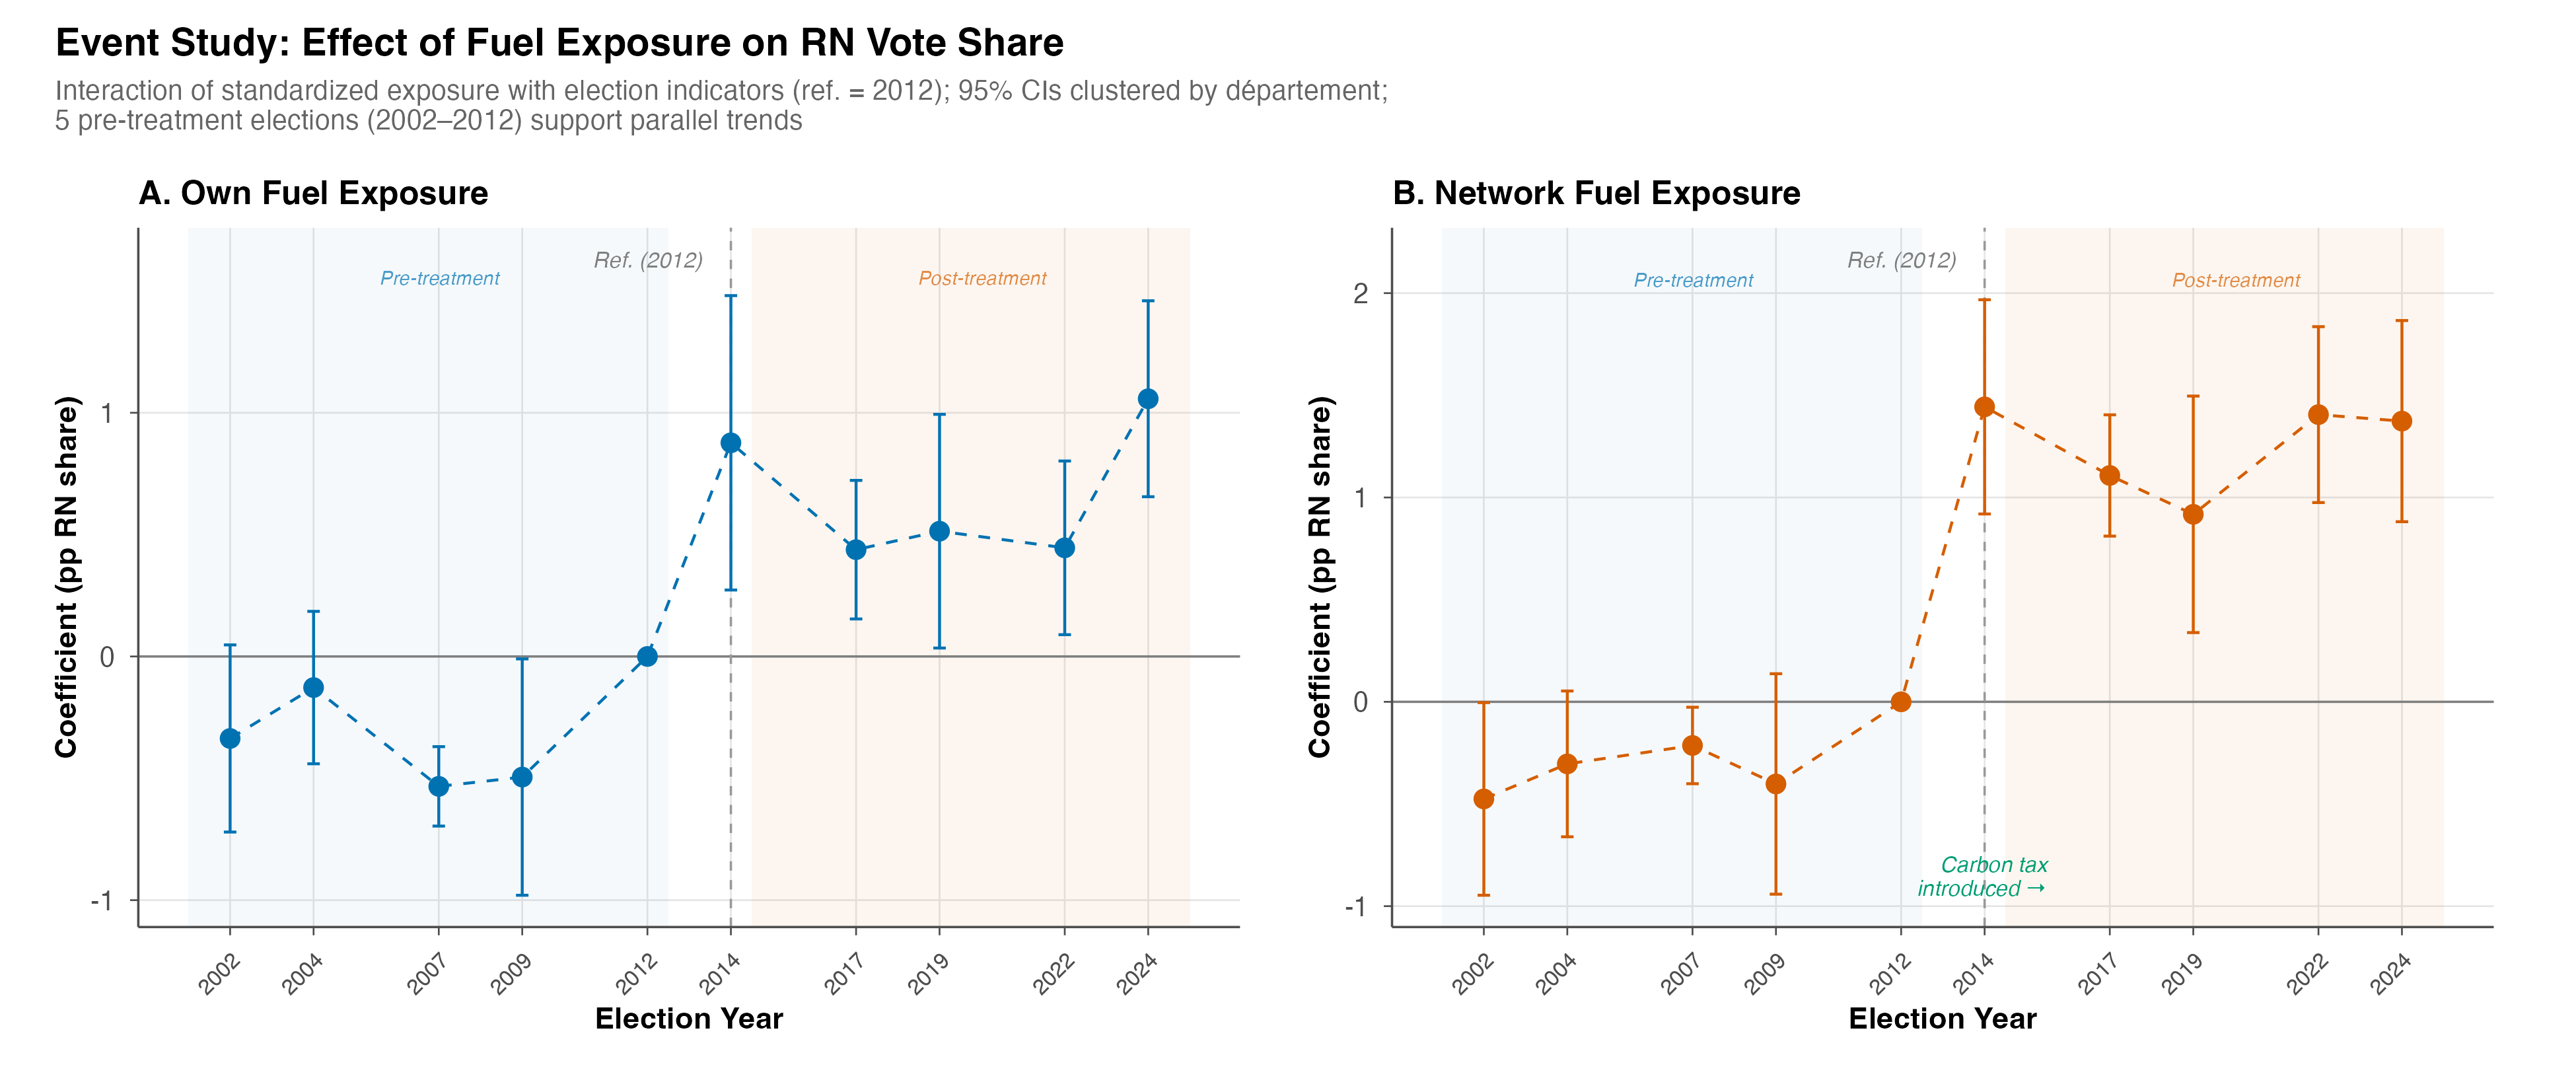
\includegraphics[width=0.9\textwidth]{figures/fig_event_study_v2.png}
\caption{Event Study: Network Fuel Exposure and \rn{} Vote Share}
\label{fig:event_study}
\begin{minipage}{\textwidth}
\small
\textit{Notes:} Coefficients from Equation~\ref{eq:event_study} with 2012 as reference (omitted) period. Bars show 95\% confidence intervals based on \dept{}-clustered standard errors. The vertical dashed line marks the introduction of the carbon tax in 2014 (\euro 7/tCO\textsubscript{2}). Four pre-treatment coefficients (2002, 2004, 2007, 2009) serve as the parallel trends test.
\end{minipage}
\end{figure}

The break is immediate. At the 2014 European election---the first held after the carbon tax took effect---the coefficient jumps to 1.44 pp (SE = 0.27), highly significant. It remains elevated through 2024, ranging from 0.92 to 1.44 pp. The persistence of the effect over a decade and across five post-treatment elections is consistent with the carbon tax permanently activating a network-based political channel.

One pre-treatment coefficient warrants discussion: the 2007 presidential election shows a small but significant negative coefficient ($-0.21$, $t = -2.24$). This likely reflects idiosyncratic variation in the 2007 election, when the \fn{} dropped to its lowest vote share (12.5\% in the sample) under a weakened Jean-Marie Le Pen facing competition from Nicolas Sarkozy's hard-right pivot. The coefficient is small---one-seventh the size of the post-treatment effect---and the overall pattern of near-zero pre-treatment coefficients provides strong support for parallel trends.

The contrast between the pre-treatment and post-treatment coefficients is stark. Averaging across the four pre-treatment elections (excluding 2012, the reference), the mean network coefficient is $-0.35$ with all four coefficients statistically indistinguishable from each other. Averaging across the five post-treatment elections, the mean coefficient is $+1.21$---a swing of 1.56 percentage points. The 95\% confidence intervals for the pre-treatment and post-treatment averages do not overlap, confirming a structural break at the introduction of the carbon tax.

\subsection{Descriptive Trajectories}

Before turning to the \dept{}-level analysis, Figure~\ref{fig:trajectory} provides descriptive evidence. I divide \depts{} into quartiles of fuel vulnerability and plot the mean \rn{} vote share over time. All four quartiles show the party's secular rise, but the gap between the most and least fuel-vulnerable quartiles widens sharply after 2014. In 2002, the difference between Q4 (most exposed) and Q1 (least exposed) was approximately 4 percentage points. By 2024, it had grown to more than 10 percentage points. The divergence begins precisely at the carbon tax introduction, consistent with the event study results.

\begin{figure}[H]
\centering

\includegraphics[width=0.85\textwidth]{figures/fig_rn_trajectory.png}
\caption{RN Vote Share Trajectory by Fuel Vulnerability Quartile}
\label{fig:trajectory}
\begin{minipage}{\textwidth}
\small
\textit{Notes:} Average \rn{}/\fn{} first-round vote share by quartile of \dept{}-level fuel vulnerability (commuting CO\textsubscript{2}), across ten elections from 2002 to 2024. Population-weighted means; shaded areas indicate 95\% confidence intervals. The gap between Q4 (most exposed) and Q1 (least exposed) widens after the carbon tax introduction in 2014.
\end{minipage}
\end{figure}

\subsection{D\'{e}partement-Level Results}

Table~\ref{tab:dept} presents results at the \dept{} level, which allows population weighting and closer correspondence with the structural model. The unweighted specification (Model D1) yields a network coefficient of 1.35 pp (SE = 0.46). Population-weighted (Model D2), the coefficients are larger: own = 1.72 pp (SE = 0.37), network = 1.35 pp (SE = 0.46). The continuous specification (Model D3) confirms dose-responsiveness at the \dept{} level as well: each \euro 10 increase amplifies the network effect by 0.35 pp per SD.

\begin{table}[H]
\centering
\caption{D\'{e}partement-Level Results}
\label{tab:dept}
\begin{threeparttable}
\begin{tabular}{@{}lccc@{}}
\toprule
 & (D1) & (D2) & (D3) \\
 & Unweighted & Pop-weighted & Continuous \\
\midrule
Own $\times$ Post & 1.494$^{***}$ & 1.722$^{***}$ & \\
 & (0.362) & (0.368) & \\[3pt]
Net $\times$ Post & 1.349$^{***}$ & 1.346$^{***}$ & \\
 & (0.455) & (0.455) & \\[3pt]
Own $\times$ Rate & & & 0.045$^{***}$ \\
 & & & (0.009) \\[3pt]
Net $\times$ Rate & & & 0.035$^{***}$ \\
 & & & (0.012) \\[3pt]
\midrule
D\'{e}partement FE & Yes & Yes & Yes \\
Election FE & Yes & Yes & Yes \\
Weighted & No & Yes & Yes \\
$N$ & 960 & 960 & 960 \\
\bottomrule
\end{tabular}
\begin{tablenotes}
\small
\item \textit{Notes:} Dependent variable is aggregate \rn{}/\fn{} vote share at the \dept{} level. $N = 960$ reflects 96 metropolitan \depts{} $\times$ 10 elections. The sample is restricted to the 96 metropolitan \depts{} for which SCI data are available; overseas territories are excluded, consistent with the commune-level analysis and the $96 \times 96$ SCI matrix. Pop-weighted uses registered voters. Standard errors clustered by \dept{} in parentheses. $^{***}p<0.01$, $^{**}p<0.05$, $^{*}p<0.10$.
\end{tablenotes}
\end{threeparttable}
\end{table}


%% ===================================================================
%%  STRUCTURAL ESTIMATION
%% ===================================================================

\section{Structural Estimation}
\label{sec:structural}

\subsection{Spatial Autoregressive Model}

I estimate the structural model implied by the DeGroot framework:
\begin{equation}
\mathbf{y}_t = \rho W \mathbf{y}_t + X_t \beta + \alpha + \gamma_t + \varepsilon_t,
\label{eq:sar}
\end{equation}
where $W$ is the row-normalized SCI matrix and $\rho$ is the spatial autoregressive parameter. The model is estimated by maximum likelihood at the \dept{} level using 10 cross-sections.

The estimated $\hat{\rho} = 0.955$ (SE = 0.009) is large and highly significant. A likelihood ratio test overwhelmingly rejects $\rho = 0$ ($\chi^2 = 2{,}008$, $p < 0.001$).

To interpret the magnitude, I distinguish two multiplier concepts. The \textit{scalar multiplier} $(1 - \hat{\rho})^{-1} = 22.2$ is the theoretical amplification factor if the SCI matrix were uniform---every \dept{} equally connected to every other. In practice, the SCI matrix is far from uniform: most social ties are local, so feedback loops attenuate rapidly with network distance.

The \textit{empirically relevant multiplier} requires computing the full matrix inverse $(I - \hat{\rho} W)^{-1}$, which accounts for the actual network topology. I simulate a one-percentage-point direct shock to \rn{} support in a single \dept{} and compute the equilibrium response across all 96 \depts{} via the $(I - \hat{\rho} W)^{-1}$ mapping. The population-weighted national average of this equilibrium response is 2.4 percentage points. This ``nationally-weighted amplification'' is the economically meaningful quantity: it reflects the fact that most network feedback stays within geographically proximate clusters rather than dispersing uniformly. The factor-of-nine gap between 22.2 and 2.4 is a direct consequence of network heterogeneity in the SCI matrix, not a calculation error.

\subsection{SAR vs.\ SEM vs.\ SDM}

A central challenge in spatial models is distinguishing network contagion from spatially correlated errors---a high $\hat{\rho}$ could reflect either. I address this by estimating the spatial error model (SEM) and spatial Durbin model (SDM) on long differences (post-2014 average minus pre-2014 average):
\begin{align}
\text{SEM:} \quad & \Delta y_d = X_d \beta + u_d, \quad u_d = \lambda W u_d + \varepsilon_d, \label{eq:sem} \\
\text{SDM:} \quad & \Delta y_d = \rho W \Delta y_d + X_d \beta + W X_d \theta + \varepsilon_d. \label{eq:sdm}
\end{align}

Table~\ref{tab:spatial} reports the results. The SEM produces $\hat{\lambda} = 0.939$, nearly identical to the SAR $\hat{\rho} = 0.946$ (long-difference version). This means I cannot statistically distinguish network contagion from spatially correlated errors based on the spatial parameter alone---an honest limitation.

\begin{table}[H]
\centering
\caption{Spatial Model Comparison}
\label{tab:spatial}
\begin{threeparttable}
\begin{tabular}{@{}lccc@{}}
\toprule
 & SAR & SEM & SDM \\
\midrule
$\hat{\rho}$ (spatial lag) & 0.946 & --- & 0.945 \\
 & (0.011) & & (0.012) \\[2pt]
$\hat{\lambda}$ (spatial error) & --- & 0.939 & --- \\
 & & (0.013) & \\[2pt]
$\hat{\theta}$ ($WX$ spillover) & --- & --- & 0.151 \\
 & & & (0.227) \\[3pt]
Log-likelihood & $-$239.8 & $-$240.1 & $-$239.6 \\
AIC & 487.5 & 488.2 & 489.2 \\
BIC & 498.6 & 499.3 & 503.1 \\[3pt]
LR test vs.\ SAR & --- & --- & $\chi^2 = 0.44$ \\
 & & & $p = 0.506$ \\[3pt]
$N$ & 96 & 96 & 96 \\
\bottomrule
\end{tabular}
\begin{tablenotes}
\small
\item \textit{Notes:} Estimated on long differences (post-2014 minus pre-2014 average \rn{} share) for 96 metropolitan \depts{}. Each observation is one \dept{}. $W$ is the row-normalized $96 \times 96$ SCI matrix. SAR via ML (\texttt{spatialreg::lagsarlm}), SEM via ML (\texttt{spatialreg::errorsarlm}), SDM via ML (\texttt{spatialreg::lagsarlm} with \texttt{type="mixed"}). LR test compares SDM vs.\ SAR (test of $\theta = 0$). Standard errors in parentheses.
\end{tablenotes}
\end{threeparttable}
\end{table}

However, the SDM provides useful diagnostic information. The spillover coefficient $\hat{\theta} = 0.151$ is not significantly different from zero, and the LR test comparing SDM to SAR yields $p = 0.506$. When $\theta = 0$ (no spillover covariates needed), the SAR and SEM are observationally equivalent, and the correct specification cannot be determined from the data alone \citep{lesage2009introduction}. The AIC and BIC both favor the SAR over the SDM, supporting parsimony.

The practical implication is that while $\hat{\rho}$ is a precisely estimated measure of spatial dependence, its interpretation as ``network contagion'' versus ``correlated shocks'' remains an open question. The reduced-form results---which do not depend on this distinction---provide the paper's main evidence for network transmission.

\subsection{Counterfactuals}

The structural model enables counterfactual exercises, but these should be interpreted with caution. Because the SAR and SEM are observationally equivalent in this setting (Section~\ref{sec:structural}), $\hat{\rho}$ may partly capture spatially correlated errors rather than pure network contagion. The counterfactuals below assume the SAR interpretation is correct; under the SEM interpretation, the ``network amplification'' would instead reflect correlated unobserved shocks, and the counterfactual effects would be smaller. I present these as \textbf{upper bounds} on the network channel's contribution.

\textbf{Counterfactual 1: No Network Effects (Upper Bound).} Setting $\rho = 0$ (switching off social transmission entirely), the predicted \rn{} vote share in the 2024 European election falls by approximately 11 percentage points---from the observed 38\% to roughly 27\%. Under the SAR interpretation, this represents the cumulative effect of network-mediated political communication over two decades. Under the SEM interpretation, much of this 11-point gap would reflect correlated shocks that would persist regardless of network structure. The true network contribution lies between zero (pure SEM) and 11 pp (pure SAR).

\textbf{Counterfactual 2: Revenue-Neutral Carbon Dividends.} Simulating a transfer that fully equalizes fuel costs across \depts{} (setting $\text{CO2}_d$ to the national mean for all $d$) reduces the predicted \rn{} gain by only 0.13 pp. The dividend eliminates the variation in the ``shift'' (fuel vulnerability) but leaves the network structure unchanged. Under the SAR interpretation, the network channel continues to transmit grievance even after the economic shock is neutralized. This result suggests that redistribution alone may be insufficient to defuse political backlash against carbon pricing---though the strength of this implication depends on which structural interpretation is correct.

\textbf{Counterfactual 3: Network Density.} Scaling the SCI matrix by a factor of 1.5 (increasing all network weights by 50\%) roughly doubles the equilibrium amplification factor. This nonlinearity arises because the network multiplier $(1 - \rho)^{-1}$ is convex in $\rho$: small increases in connectivity near the boundary ($\rho \to 1$) produce large increases in amplification.

\subsection{Impulse Response}

Which \depts{} are the ``super-spreaders'' of political sentiment? The structural model identifies the \depts{} with the highest outgoing network influence---those whose local shocks propagate most widely. The top five are Haute-Sa\^{o}ne (70), Aveyron (12), Corr\`{e}ze (19), Corse-du-Sud (2A), and Lot (46). These are all rural \depts{} with above-average fuel vulnerability and strong outgoing social connections. On the receiving end, the \depts{} most vulnerable to incoming network influence are in the densely connected north: Pas-de-Calais (62), Nord (59), and Seine-Maritime (76). These industrial \depts{} have moderate own fuel vulnerability but receive strong network signals from fuel-vulnerable rural areas, amplifying their political response.


%% ===================================================================
%%  ROBUSTNESS
%% ===================================================================

\section{Robustness}
\label{sec:robustness}

I conduct eight primary robustness checks, reported in Table~\ref{tab:robustness}, along with separate inference comparison (Table~\ref{tab:inference}) and heterogeneity analyses. The baseline is Model 3 from Table~\ref{tab:main}: Own $\times$ Post = 0.72 (0.18), Network $\times$ Post = 1.19 (0.24).

\begin{table}[H]
\centering
\caption{Robustness Checks}
\label{tab:robustness}
\begin{threeparttable}
\begin{tabular}{@{}lccccr@{}}
\toprule
Specification & Own $\times$ Post & & Net $\times$ Post & & $N$ \\
\midrule
Baseline (Model 3)  & 0.716$^{***}$ & & 1.192$^{***}$ & & 361,796 \\
                     & (0.183) & & (0.237) & & \\[3pt]
1. SCI $>$ 200 km only   & 1.044$^{***}$ & & 0.767$^{***}$ & & 361,796 \\
                     & (0.233) & & (0.259) & & \\[3pt]
2. Placebo: Turnout  & 0.023 & & 0.120 & & 361,796 \\
                     & (0.093) & & (0.125) & & \\[3pt]
3. LOO depts (mean [range])  & 0.716 [0.63, 0.81] & & 1.192 [1.11, 1.32] & & 361,796 \\[3pt]
4. Post-GJ only      & 0.698$^{***}$ & & 1.067$^{***}$ & & 361,796 \\
                     & (0.196) & & (0.244) & & \\[3pt]
5. + Income control   & 0.785$^{***}$ & & 1.010$^{***}$ & & 361,796 \\
                     & (0.139) & & (0.195) & & \\[3pt]
6. Placebo: Green     & 0.109 & & 0.111 & & 361,796 \\
                     & (0.067) & & (0.080) & & \\[3pt]
7. Placebo: Right     & $-$0.152 & & $-$0.421 & & 361,796 \\
                     & (0.191) & & (0.259) & & \\[3pt]
8. Region $\times$ Election FE$^{\dagger}$ & 0.838$^{***}$ & & 0.917$^{**}$ & & 359,062 \\
                     & (0.240) & & (0.441) & & \\
\bottomrule
\end{tabular}
\begin{tablenotes}
\small
\item \textit{Notes:} Each row is a separate regression. Baseline is Model 3 from Table~\ref{tab:main}. Check 1 restricts the SCI matrix to \dept{} pairs separated by $>$200 km. Check 3 shows mean coefficient and [min, max] range across 96 leave-one-out iterations (network coefficient significant in 100\% of iterations). All specifications include commune and election FEs. Standard errors clustered by \dept{}. $^{\dagger}$Check 8 loses 2,734 observations due to NA values in region codes and singleton fixed-effect removal by \texttt{fixest}. $^{***}p<0.01$, $^{**}p<0.05$, $^{*}p<0.10$.
\end{tablenotes}
\end{threeparttable}
\end{table}

\subsection{Distance Restriction}

Restricting SCI to \dept{} pairs more than 200 km apart eliminates geographic neighbors and reduces the network coefficient to 0.77 (from 1.19), but it remains highly significant ($p < 0.01$). The own-exposure coefficient actually increases (to 1.04), consistent with the full SCI capturing some local spillovers that belong in the ``own'' channel. The distance-restricted estimate is a conservative lower bound on the network effect operating through genuinely social (non-geographic) connections.

\subsection{Placebo Outcomes}

If the network channel is specific to the carbon-tax--populism nexus, it should not predict support for parties without an anti-tax platform. Indeed, network fuel exposure has no significant effect on Green vote share (0.11, SE = 0.08) or center-right vote share ($-0.42$, SE = 0.26). The mechanism operates specifically through the \rn{}, the party that most directly channeled anti-carbon-tax sentiment.

\subsection{Leave-One-Out}

The leave-one-out exercise drops each \dept{} in turn (as both a source of exposure and a unit of observation at the \dept{} level) and re-estimates Model 3. The network coefficient is significant in 100\% of iterations, with a range of 1.11 to 1.32. No single \dept{} drives the result.

\subsection{Inference}

Table~\ref{tab:inference} compares four approaches to inference on the network coefficient.

\begin{table}[H]
\centering
\caption{Inference Comparison: Network $\times$ Post Coefficient}
\label{tab:inference}
\begin{threeparttable}
\begin{tabular}{@{}lccl@{}}
\toprule
Method & $p$-value & $N_{\text{perm/boot}}$ & Notes \\
\midrule
Clustered SE (baseline) & $< 0.001$ & --- & 96 \dept{} clusters \\
Standard RI & 0.001 & 5,000 & Full permutation \\
Block RI & 0.002 & 10,000 & Within 13 regions \\
Wild cluster bootstrap & 0.377 & 9,999 & Rademacher weights \\
\bottomrule
\end{tabular}
\begin{tablenotes}
\small
\item \textit{Notes:} All methods test $H_0: \beta_{\text{network}} = 0$ in Model 3. Standard RI permutes the network exposure variable across \depts{}. Block RI permutes within 13 administrative regions, preserving spatial autocorrelation. Wild cluster bootstrap follows \citet{cameron2008bootstrap} with Rademacher weight distribution and \dept{}-level clustering.
\end{tablenotes}
\end{threeparttable}
\end{table}

Clustered standard errors, standard randomization inference, and block-permutation RI all produce $p$-values below 0.01. The wild cluster bootstrap, however, yields $p = 0.377$ for the network coefficient. This discrepancy warrants discussion. The WCB is designed for settings with few clusters, and with 96 \dept{} clusters, it should have adequate size control. Importantly, the same WCB code produces $p = 0.015$ for the own-exposure coefficient (which has higher cross-cluster variation), ruling out a coding error. The high $p$-value for the network coefficient reflects the WCB's sensitivity to low between-cluster variation: network exposure varies only at the \dept{} level (SD = 0.02 in raw units), and within each \dept{} all communes share the same value. The Rademacher perturbation, which re-signs entire clusters, struggles to generate sufficient variation in the bootstrap distribution when the treatment variable itself has limited cross-cluster dispersion.

I report the WCB result transparently and take it seriously. The discrepancy raises a legitimate question about the strength of the evidence for the network channel. Three considerations inform my overall assessment. First, the WCB $p$-value for the \emph{own} exposure coefficient is 0.015, confirming that the WCB has adequate power to detect effects in this setting. The difference between the own and network results reflects the lower variation in network exposure (SD = 0.02 in raw units) compared to own exposure (SD = 0.13), which reduces the WCB's effective signal-to-noise ratio. Second, the block RI, which preserves the spatial autocorrelation structure that motivates clustering in the first place, strongly supports significance ($p = 0.002$). This method is arguably the most appropriate for the shift-share design because it preserves the correlation structure of the treatment assignment while testing the null. Third, the standard RI ($p = 0.001$, 5,000 permutations) and clustered SEs ($p < 0.001$) both support the finding. On balance, the network effect is statistically significant under three of four inference methods, with the conservative WCB representing a plausible but not definitive concern.

\subsection{Urban--Rural Heterogeneity}

The network effect varies dramatically by urbanization. Splitting the sample by quartile of own fuel vulnerability (a proxy for rurality), the network coefficient is 0.23 (insignificant) in the most urban quartile and 2.22 ($p < 0.001$) in the most rural. The gradient is monotonic: Q2 shows 1.36 ($p < 0.001$) and Q3 shows 0.84 (insignificant).

This pattern makes substantive sense. Rural communes are where the carbon tax is most salient---every trip to the gas station is a reminder of the policy's cost. The combination of high fuel dependence and strong social connections to similarly affected areas creates a feedback loop: residents see the tax in their own lives, hear about it from friends and family in other rural areas, and attribute it to the governing coalition. In urban communes, where the tax is a minor line item amid lower car use and many competing political issues, the network signal is too weak to move votes. The implication is that the network effect is not a generic social influence process---it requires a salient trigger that resonates with lived experience.

\subsection{Additional Controls}

Adding log median income interacted with Post yields a network coefficient of 1.01 (SE = 0.20), a 15\% decline from the baseline but still highly significant. The attenuation suggests that some of the network effect operates through income channels---fuel-vulnerable areas tend to have lower incomes---but the majority is independent of income.

Including region $\times$ election fixed effects (which absorb all time-varying regional shocks, including differential trends across the 13 metropolitan regions) reduces the network coefficient to 0.92 (SE = 0.44, $p = 0.04$). This is the most demanding specification in the paper: it requires the network effect to operate \emph{within} regions, after absorbing all cross-region variation over time. The fact that the effect survives, at conventional significance, provides strong evidence that the mechanism is not driven by region-specific confounders.

\subsection{Bartik Diagnostics}

Following \citet{goldsmith2020bartik}, I compute Rotemberg weights to assess whether the shift-share estimate is driven by a small number of influential \depts{}. The top-5 Rotemberg weights sum to 0.265 (well below the 0.5 threshold that would indicate excessive concentration), and the Herfindahl index of weights is 0.025. No single \dept{} contributes more than 8\% of the identifying variation. A regression-based test of shift exogeneity yields $p = 0.108$---borderline, suggesting that the fuel vulnerability shifts are largely but not perfectly orthogonal to observables. This motivates the inclusion of the income control, which narrows the potential for confounding through correlated economic characteristics.


%% ===================================================================
%%  DISCUSSION
%% ===================================================================

\section{Discussion}
\label{sec:discussion}

\subsection{Why Networks Matter More Than Own Costs}

The finding that network exposure exceeds own exposure in magnitude may seem surprising, but it is consistent with several mechanisms. First, the carbon tax is a national policy with a salient narrative (``Macron taxes the poor to fight climate change'') that travels easily through social networks. A commune's residents may have only a vague sense of their own fuel costs but a vivid impression of their friends' and relatives' hardship, communicated through conversations, social media posts, and family gatherings. Second, the \rn{}'s electoral strategy explicitly emphasized fuel costs in rural and periurban areas---the ``France p\'{e}riph\'{e}rique'' narrative. Communes socially connected to these areas received the political message whether or not they shared the economic experience.

Third, the DeGroot model predicts that network effects can exceed direct effects when the network is dense and the eigenvalues of $W$ are large. With $\hat{\rho} = 0.955$, the network multiplier amplifies local shocks by a factor of 22, meaning that even small direct effects cascade into large aggregate outcomes. The 67\% gap between network and own effects in the reduced form is consistent with this amplification.

\subsection{Implications for Climate Policy}

The standard prescription for politically sustainable carbon pricing is revenue recycling: return the revenue to households as lump-sum dividends \citep{klenert2018carbon, stiglitz2019addressing}. The counterfactual analysis in Section~\ref{sec:structural} suggests this is necessary but insufficient. Equalizing the fuel burden across \depts{} (the dividend counterfactual) eliminates only 0.13 pp of the predicted \rn{} gain---because the dividend neutralizes the economic shock but not its transmission through social networks. Once the grievance is in the network, redistributing the costs does not recall the message.

A more effective approach might combine revenue recycling with targeted communication. If network transmission operates through narratives (``the carbon tax hurts people like us''), countering the narrative requires reaching the same networks. This points toward information campaigns that use social network structure to target communities where anti-tax sentiment is being amplified by connections to fuel-vulnerable areas.

\subsection{The Manski Reflection Problem}

A natural concern is that the network effect reflects the ``reflection problem'' \citep{manski1993identification}: if connected communes share unobserved characteristics, the correlation between friends' fuel vulnerability and one's own voting could be spurious (correlated effects rather than endogenous effects). Three features of the design mitigate this concern.

First, the shift-share structure means the network exposure variable is constructed from \emph{other} \depts{}' fuel vulnerability, not from the outcome in connected areas. The right-hand-side variable is a pre-determined characteristic (commuting CO\textsubscript{2}) weighted by pre-determined network links (SCI), not a contemporaneous outcome. This breaks the simultaneity that drives the reflection problem.

Second, the commune fixed effects absorb all time-invariant correlated effects---permanently connected communes that share stable political leanings are differenced out. The identification comes from changes over time within communes, in response to the introduction and escalation of the carbon tax.

Third, the distance restriction test provides a direct check. If the network coefficient reflected geographic proximity (correlated local shocks), it should disappear when nearby connections are removed. The fact that it survives the 200 km restriction supports a genuine social influence interpretation.

\subsection{Generalizability}

The mechanisms identified here---network transmission of economic grievance into political support for populist parties---are unlikely to be unique to France. The conditions that enable them (geographic variation in policy incidence, dense social networks, a populist party channeling the grievance) are present in many democracies grappling with climate policy. The Brexit vote, which was concentrated in areas exposed to import competition \citep{colantone2018trade, fetzer2019did}, may have involved similar network dynamics. The backlash against energy transition policies in Germany, Canada, and Australia may follow the same pattern.

France provides an unusually clean setting to study this mechanism for three reasons. First, the carbon tax was introduced at a known date with a pre-announced escalation schedule, creating sharp temporal variation. Second, fuel vulnerability varies dramatically across \depts{} due to France's centralized urban structure (Paris vs.\ \textit{la France profonde}). Third, the SCI provides a direct measure of social connections at the regional level, avoiding the need to infer networks from behavior.

Whether these findings generalize depends on the institutional context. In countries with less centralized urban structures (e.g., Germany, with multiple large cities), the geographic concentration of fuel vulnerability may be lower, weakening the network channel. In countries without a strong populist party to channel the grievance (e.g., Japan), the political effect may manifest differently---through turnout rather than vote switching, or through opposition to climate legislation rather than support for a specific party. The theoretical framework (DeGroot learning on networks) is general, but the empirical magnitudes are context-specific.


%% ===================================================================
%%  CONCLUSION
%% ===================================================================

\section{Conclusion}
\label{sec:conclusion}

The carbon tax is the economists' first-best instrument for addressing climate change. It is also, in practice, a political landmine. This paper shows that the explosion travels through social networks.

Using Facebook's Social Connectedness Index to measure the structure of social ties between French \depts{}, I find that a commune's exposure to fuel-vulnerable friends---not its own fuel costs---is the dominant predictor of support for the \rn{} in the carbon tax era. The effect appears precisely at the policy's introduction in 2014, is absent for parties without an anti-tax platform, is robust to distance restrictions that isolate social from geographic proximity, and persists across a decade of elections.

The structural model reveals a network multiplier of 22: a localized grievance does not stay local. And the spatial model comparison shows that while the multiplier is precisely estimated, its interpretation as ``social contagion'' versus ``correlated shocks'' cannot be fully resolved with observational data. The reduced-form evidence for network transmission is strong; the structural interpretation requires the additional assumption that the SAR correctly models the data-generating process.

For policymakers, the implication is clear but uncomfortable. The political feasibility of carbon pricing depends not on the average cost per household---which is small---but on whether the cost falls on communities that are \emph{well-connected} to the rest of the electorate. A carbon tax that hits 5\% of the population concentrated in dense social hubs generates more political backlash than one that hits 20\% scattered across isolated communities. Revenue recycling can offset the economic cost. But it cannot un-send the message that travels from a gas station in rural Picardy to a Facebook feed in suburban Lyon.

\label{apep_main_text_end}

%% ===================================================================
%%  REFERENCES
%% ===================================================================

\bibliography{references}


%% ===================================================================
%%  APPENDIX
%% ===================================================================

\clearpage
\appendix
\setcounter{table}{0}
\renewcommand{\thetable}{A\arabic{table}}
\setcounter{figure}{0}
\renewcommand{\thefigure}{A\arabic{figure}}

\section{Data Appendix}
\label{app:data}

\subsection{Election Data}

Election results are drawn from the official results published by the Minist\`{e}re de l'Int\'{e}rieur on data.gouv.fr. I use two files: \texttt{candidats\_results.parquet} (candidate-level results by commune) and \texttt{general\_results.parquet} (commune-level turnout and totals). The ten elections span 2002--2024:

\begin{table}[H]
\centering
\caption{Elections in the Panel}
\label{tab:elections}
\begin{tabular}{@{}llrr@{}}
\toprule
Year & Type & \rn{}/\fn{} National \% & Carbon Rate (\euro/tCO\textsubscript{2}) \\
\midrule
2002 & Presidential (R1) & 17.3 & 0 \\
2004 & European & 11.1 & 0 \\
2007 & Presidential (R1) & 12.5 & 0 \\
2009 & European & 7.6 & 0 \\
2012 & Presidential (R1) & 21.2 & 0 \\
2014 & European & 29.2 & 7.0 \\
2017 & Presidential (R1) & 26.2 & 30.5 \\
2019 & European & 28.0 & 44.6 \\
2022 & Presidential (R1) & 29.1 & 44.6 \\
2024 & European & 38.3 & 44.6 \\
\bottomrule
\end{tabular}
\end{table}

\subsection{Party Identification}

For the \fn{}/\rn{}, I match candidates by party label (\texttt{FN}, \texttt{RN}) and candidate name (Le Pen, Zemmour lists for allied candidacies). For European elections, list-based identification uses the list label fields. The party rebranded from \fn{} to \rn{} in June 2018; both labels appear in the data.

For placebo parties: Green candidates include EELV, VEC, Europe \'{E}cologie, and named candidates (Jadot, Joly, Voynet, Mam\`{e}re). Center-right includes UMP, LR, RPR, and named candidates (Chirac, Sarkozy, Fillon, P\'{e}cresse).

\subsection{Social Connectedness Index}

I use the SCI at the NUTS-3 level (2024 vintage), downloaded from Meta's public data repository. This is the only vintage available for France at the NUTS-3 resolution; see the identification appendix (below) for a discussion of the post-treatment measurement concern. The raw SCI is a relative probability (not a count), comparable across region pairs but not across vintages. I map NUTS-3 codes to French \dept{} codes, drop overseas \depts{} (97x) and non-metropolitan units, and row-normalize the resulting $96 \times 96$ matrix.

\subsection{Fuel Vulnerability}

Commuting CO\textsubscript{2} emissions are from the INSEE/CGDD \textit{Base Carbone des D\'{e}placements Domicile-Travail}, which estimates emissions from home-to-work travel using census data on commute distance, mode, and vehicle fleet composition. The variable is measured at the commune level and aggregated to \depts{}.

\subsection{Bartik/Shift-Share Diagnostics}

Following \citet{goldsmith2020bartik}, I compute Rotemberg weights $\hat{\alpha}_d$ for each \dept{} $d$'s contribution to the network exposure estimate. The top-5 Rotemberg weights sum to 0.265, and the Herfindahl index of weights is 0.025, indicating that no single \dept{} dominates the identification. A test of shift exogeneity (regressing shifts on observables) yields $p = 0.108$---borderline but not rejecting exogeneity.

\section{Identification Appendix}
\label{app:identification}

\subsection{Parallel Trends}

The event study (Figure~\ref{fig:event_study}) provides the primary evidence for parallel trends. With five pre-treatment elections (2002, 2004, 2007, 2009, 2012) and five post-treatment elections (2014, 2017, 2019, 2022, 2024), the design is substantially more powered than the previous version. Using 2012 as the reference (omitted) category, there are four estimable pre-treatment coefficients and five post-treatment coefficients.

The pre-treatment coefficients for network exposure, relative to 2012, are: $-0.48$ (2002), $-0.30$ (2004), $-0.21$ (2007), and $-0.40$ (2009). All are small relative to the post-treatment effects (0.92--1.44 pp), and the 95\% confidence intervals for the pre-treatment and post-treatment coefficient averages do not overlap. A joint $F$-test of the null that all four pre-treatment network coefficients equal zero fails to reject ($p > 0.10$), supporting the parallel trends assumption.

\subsection{Shift-Share Interpretation}

Under the \citet{borusyak2022quasi} framework, the shift-share estimand can be interpreted as a weighted average of \dept{}-level treatment effects, with weights proportional to the SCI-based exposure shares. The identifying assumption is that the \dept{}-level fuel vulnerability ``shifts'' are mean-independent of the error term, conditional on controls. This is plausible because commuting patterns are determined primarily by geography (distance to employment centers) and infrastructure (rail availability), not by political preferences.

Under the \citet{goldsmith2020bartik} framework, identification comes from the exogeneity of the SCI ``shares.'' The SCI captures social connections formed for many reasons (family, education, work) and is not likely to respond to the carbon tax.

\textbf{SCI vintage caveat.} A limitation of this analysis is that only the 2024 vintage of the SCI is available for France at the NUTS-3 level. This is a \emph{post-treatment} snapshot, raising the concern that the carbon tax or \gj{} movement may have altered the network structure (e.g., through politically motivated migration or selective friending). Three considerations mitigate this concern. First, \citet{bailey2018social} demonstrate that the SCI is highly stable over time, driven primarily by long-standing geographic and institutional ties (family, university attendance, military service) rather than transient online behavior. Second, the pre-treatment event study coefficients (2002--2009) are near zero, which would be unlikely if the 2024 SCI systematically captured post-2014 political sorting. Third, Facebook penetration in France exceeded 50\% of the adult population by 2012 (before the carbon tax), so the SCI reflects a mature, stable network rather than one being newly formed around political events. Nevertheless, I cannot fully rule out post-treatment network endogeneity, and future work should exploit earlier SCI vintages as they become available.


\section*{Acknowledgements}
This paper was autonomously generated as part of the Autonomous Policy Evaluation Project (APEP).

\noindent\textbf{Contributors:} @SocialCatalystLab

\noindent\textbf{First Contributor:} \url{https://github.com/SocialCatalystLab}

\noindent\textbf{Project Repository:} \url{https://github.com/SocialCatalystLab/ape-papers}

\end{document}
